\documentclass[11pt,a4paper]{article}
\usepackage{fontspec}
\setmainfont{TeX Gyre Pagella}
\newfontfamily\headfont{Inter}[UprightFont=*-ExtraBold,BoldFont=*-ExtraBold,Extension=.otf,Path=/usr/share/fonts/opentype/inter/]
\usepackage[a4paper,margin=2.3cm]{geometry}
\usepackage{graphicx,booktabs,float,caption,array,xcolor,longtable}
\usepackage{xurl}
\usepackage[hidelinks]{hyperref}
\usepackage{titlesec}
\usepackage[round]{natbib}
\usepackage{setspace}
\setstretch{1.05}
\renewcommand{\topfraction}{0.9}
\renewcommand{\bottomfraction}{0.8}
\renewcommand{\textfraction}{0.1}
\renewcommand{\floatpagefraction}{0.75}
\setlength{\parindent}{0pt}
\setlength{\parskip}{0.55em}
\titleformat{\section}{\headfont\Large}{\thesection}{0.8em}{}
\titleformat{\subsection}{\headfont\large}{\thesubsection}{0.8em}{}
\captionsetup{font=small,labelfont=bf}
\urlstyle{same}
\hypersetup{pdftitle={Manhattanhenge for Every British Town},pdfauthor={Tristan Hotham}}

\begin{document}
\begin{center}
{\Large\bfseries Manhattanhenge for Every British Town\par}
\vspace{0.4em}
{\large When the sun rises and sets along 37,224 straight streets in 377 UK towns and cities,\\with the terrain skyline, and whether any were built for it\par}
\vspace{1.2em}
{\large Tristan Hotham\par}
\vspace{0.3em}
{\small Independent researcher\\
ORCID: 0000-0003-4931-9349\\
DOI: https://doi.org/10.5281/zenodo.24075297\par}
\vspace{0.8em}
2026
\end{center}

\begin{quote}
\small
\begin{center}\textbf{Abstract}\end{center}
Manhattanhenge is the name given to the days when the setting sun lines up with the street grid of Manhattan. I compute the equivalent days for every straight named street in the 377 towns and cities of the United Kingdom with 25,000 or more people. Named road centrelines from OpenStreetMap, read from OpenFreeMap vector tiles, are joined by name and searched for straight stretches of at least 300 m whose every vertex lies within 5.0 m of the chord (37,224 stretches, 15,638 km). For each end of each stretch the terrain skyline is computed from the AWS Terrain Tiles, and the solar declination at which the sun's centre stands on that skyline straight down the street gives the days of alignment. 49.4\% of streets line up with the rising or setting sun on at least one day a year; 1,072 lie within 1° of a solstice sunrise or sunset. Street ends within 1° of a solstice are no more frequent than a few degrees away (1.86\% against 1.83\%, ratio 1.01), so there is no national sign of design; a few towns (St Annes, Bournemouth) have more than their share because of the direction of their grids. Midsummer Boulevard in Milton Keynes, often said to be aligned with the midsummer sunrise, runs at 55.1°, 4.0° to 6.7° from the midsummer sunrise over its terrain skyline; the sun rises along it about 24 May and 20 July, and on midsummer morning it stands on the axis only when 3.6° up, about 36 minutes after sunrise, which matches the planners' own claim that it nearly lines up. Henge calendars for each town give its best days, for example 6 April and 7 September in Glasgow.

\textbf{Keywords:} street orientation; Manhattanhenge; solar alignment; urban form; OpenStreetMap; terrain horizon; archaeoastronomy
\end{quote}

\section{Introduction}
On a few evenings each year the setting sun lines up with the cross streets of Manhattan, whose grid is turned about 29° from true north, and the sun sets framed at the end of the street. The event, named Manhattanhenge by the astrophysicist Neil deGrasse Tyson, is now a fixture of the New York calendar. Any town with long straight streets has the same thing on its own dates, and some places are said to have been built for it. Milton Keynes is the British example most often given: its central avenue is called Midsummer Boulevard and is said to point at the midsummer sunrise.

This study computes the henge days of every straight named street in the UK's towns and cities, asks which streets line up with the solstices, whether that happens more often than chance, and what each town's best days are. It uses the street map of OpenStreetMap \citep{osm} through the OpenFreeMap vector tiles \citep{ofm}, the terrain of the AWS Terrain Tiles \citep{terrain} for the skyline at the end of each street, and a standard solar position \citep{spencer,bennett}. The street-orientation literature has measured the order of street grids city by city \citep{boeing}; here the question is their relation to the sun. The study accompanies an interactive map (\url{https://maps.tristanhotham.com/street-henge/}).

\section{Data}
\textbf{Towns.} Wikidata \citep{wikidata} settlements in the UK with a population of 25,000 or more and a town or city type; metropolitan areas, conurbations, counties and suburbs were removed, along with implausible populations (a suburb recorded with 2.8 million people). A town whose centre lies within three quarters of the radius of a larger town's circle was merged into it (Salford into Manchester, Gateshead into Newcastle). This leaves 377 towns. Each has a circle of radius $\sqrt{\mathrm{pop} \times 400\,\mathrm{m}^2/\pi}$, between 1.5 and 22 km.

\textbf{Streets.} For every zoom-14 tile touching a circle (9,077 tiles), the \texttt{transportation\_name} layer gives named road centrelines with their class. Trunk to minor roads, service roads, busways and pedestrian streets were kept; motorways, footpaths, cycleways and tracks were not. Each line was clipped to its own tile so that the tile buffers do not double it.

\textbf{Terrain.} AWS Terrain Tiles at zoom 10 (about 95 m cells in Britain), in the terrarium encoding.

\section{Methods}
\subsection{Straight stretches}
In each town the lines of one street name were joined end to end and searched for straight stretches: a run of vertices is straight when every vertex lies within 5.0 m of the chord joining its ends, grown greedily from each start vertex, and kept when at least 300 m long. With a 5 m tolerance the chord's direction is good to about 1° over 300 m and better over longer stretches. Two carriageways of one road (same name, bearings within 2°, less than 40 m apart side by side and overlapping) count once (2,919 removed from 40,433), and stretches that continue each other across a slight kink were joined (290 joins), giving 37,224 stretches with a median length of 372 m; 421 are a kilometre or more. Each belongs to the town whose centre is nearest. Trunk roads and anything named as a bypass, bridge, pier, viaduct, interchange, or link or relief road (3,026) are kept but flagged as roads rather than streets, and left out of the lists of henge streets; the rules are in the code's overrides file, and every solstice-aligned stretch of 600 m or more was read by name and town to check them.

\subsection{The skyline}
From each end of each stretch, looking along it towards the other end and beyond, the skyline angle is the largest elevation angle to the terrain between 100 m and 40 km, for an eye 1.7 m above the ground, with the Earth's curvature and standard refraction ($k = 0.13$). Heights are read by bilinear interpolation, replaced by the median of the nine surrounding cells where the two differ by more than 40 m (the tiles carry occasional spikes). The median skyline is 0.43°; 6.4\% of street ends have a skyline above 2°, and the highest, 13.3°, is up Ballygomartin Road, Belfast.

\subsection{The days}
For a street end looking at azimuth $A$ over a skyline of apparent altitude $h$, the sun's centre stands there when its declination is
\[\sin\delta = \sin\varphi\sin h_t + \cos\varphi\cos h_t\cos A,\]
where $h_t$ is the true altitude after removing refraction \citep{bennett} and $\varphi$ the latitude. If $|\delta| \le 23.44°$ the alignment happens on the one or two days of the year with that noon declination, from the series of \citet{spencer} for a common year (2026); the event is a sunrise if $A < 180°$ and a sunset otherwise. A street end is solstice aligned when $A$ lies within 1° (or 2°) of the azimuth of the solstice sunrise or sunset over the same skyline; ends just beyond the sun's range but within 1° count as solstice henges. The method was checked against Manhattan: a street at 299° from north at 40.75°N over a flat horizon gives 26 May and 18 July, against published dates of about 28 May and 12 July: two days out in May and six in July, a reminder that dates from a single bearing and a flat horizon are approximate to within several days near the solstices, where the sun's azimuth changes slowly.

\subsection{Chance and design}
If streets were laid out with no regard to the sun, the share of street ends within 1° of a solstice azimuth would match the share per degree a few degrees away. The expected share is the mean share per degree of offset between 2° and 8° on either side, times the 2° window, which allows for the shape of the grid and the uneven spread of street directions. The same test is run for each town with 50 or more stretches (one-sided binomial, Bonferroni corrected over 168 towns).

\subsection{Calendars and grids}
A town's henge calendar adds, for each day, the length of street that the sun rises or sets along (smoothed over a week); its best day is the peak. The town's grid direction is the length-weighted dominant direction of its stretches folded modulo 90° \citep[compare][]{boeing}, with a strength between 0 (all directions) and 1 (one direction), and the henge days of the grid are those of its four directions over a 0.5° skyline.

\section{Results}
\subsection{How many streets catch the sun}
Of 37,224 straight stretches, 18,405 (49.4\%) line up with the rising or setting sun on at least one day a year; the rest run too near north to south. Figure~\ref{fig:sun} shows the range of sunset azimuths: 232.6° to 309.1° at 50°N, 222.7° to 320.1° at 58°N.

\begin{figure}[tbp]\centering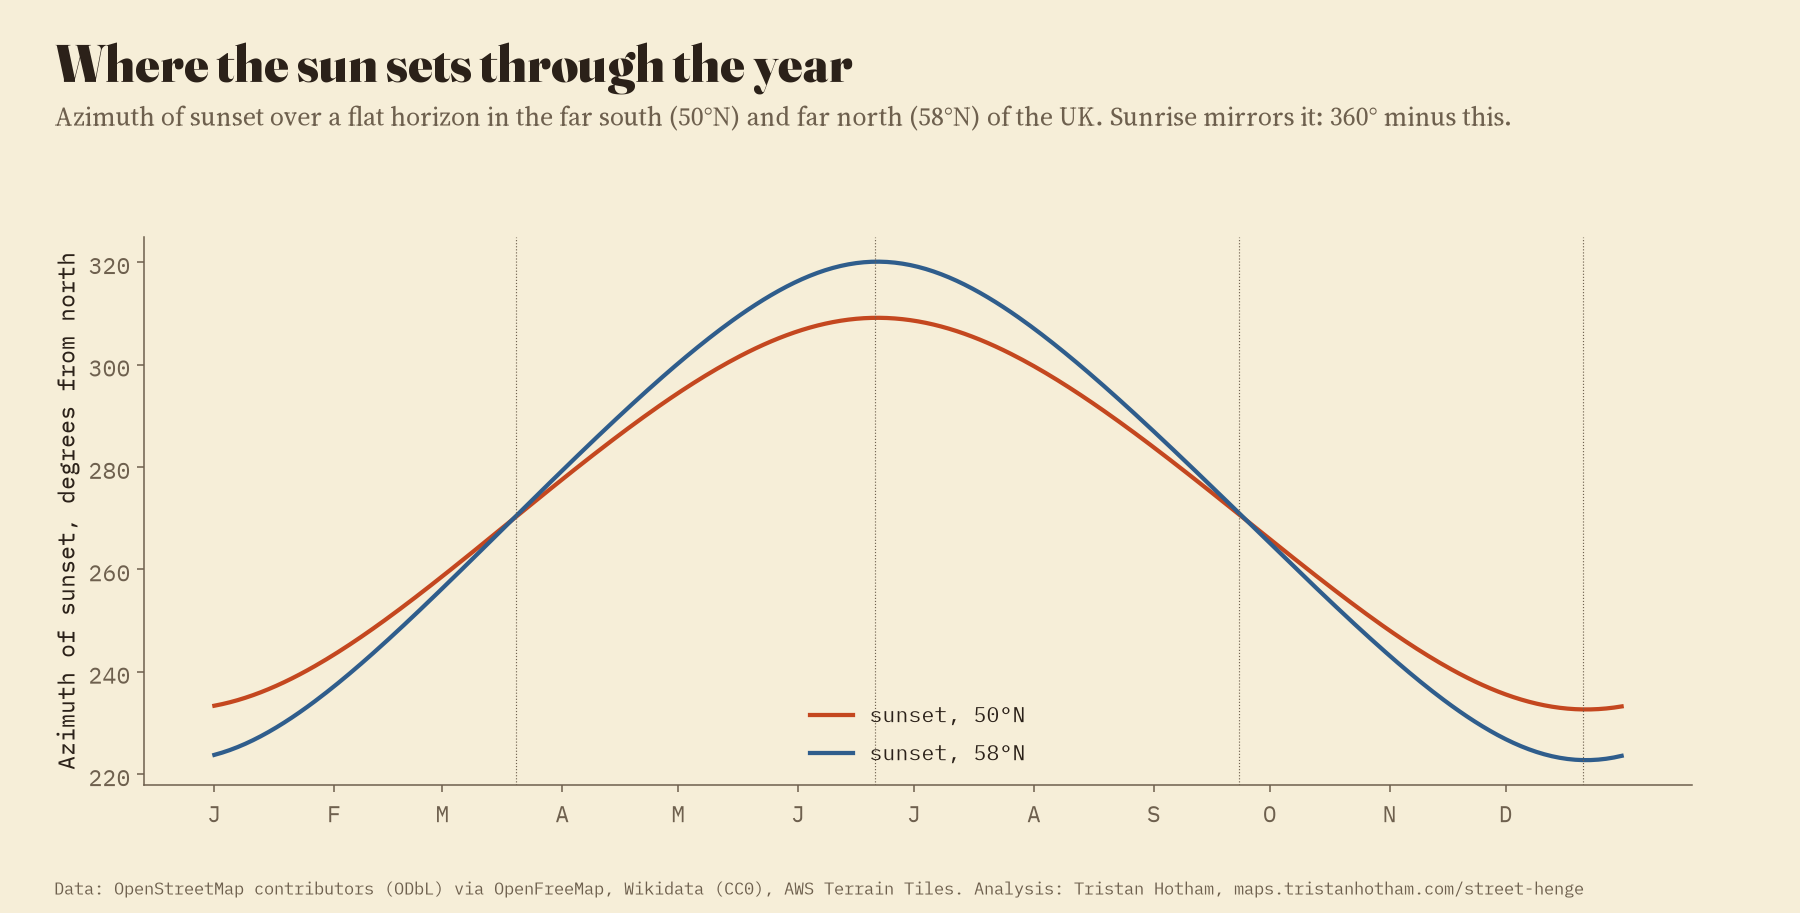
\includegraphics[width=0.9\textwidth]{f_sun.png}
\caption{Sunset azimuth through the year at 50°N and 58°N over a flat horizon.}\label{fig:sun}\end{figure}

\subsection{Solstice streets}
1,072 stretches lie within 1° of a solstice sunrise or sunset and 1,849 within 2° (Figure~\ref{fig:map}); 983 of the first are streets rather than roads, in 256 towns. 311 line up at both ends, typically with the midsummer sunrise one way and the midwinter sunset the other, the axis of Stonehenge. The longest (Table~\ref{tab:best}, Figure~\ref{fig:best}) is Bursledon Road in Southampton (2,995 m, midwinter sunrise). By event, 368 street ends face the midsummer sunrise, 325 the midsummer sunset, 310 the midwinter sunrise and 380 the midwinter sunset. Of the 105 stretches on streets named after Roman roads (54.4 km, the longest Ermine Street in Lincoln, 1,462 m), 3 line up with a solstice.

\begin{table}[tbp]\centering\footnotesize\caption{The longest straight streets within 1° of a solstice sunrise or sunset over their own skyline (trunk roads and bypasses excluded): length (m), bearing of the stretch (degrees from north, 0 to 180), the event, the offset from the solstice azimuth and the skyline angle (degrees) at the aligned end.}\label{tab:best}\begin{tabular}{llrrlrr}\toprule Street & Town & Length & Bearing & Aligned with & Offset & Skyline\\\midrule
Bursledon Road & Southampton & 2,995 & 127.8 & midwinter sunrise & 0.53 & 0.05\\
City Road & Birmingham & 1,365 & 47.9 & midsummer sunrise (both) & 0.08 & -0.19\\
Asquith Avenue & Morley & 1,139 & 132.7 & midsummer sunset & 0.94 & 0.71\\
Hertford Road & Welwyn Garden City & 1,115 & 129.6 & midwinter sunrise (both) & 0.12 & 0.20\\
Long Cross & Bristol & 1,100 & 50.0 & midwinter sunset (both) & 0.40 & 0.86\\
St Alban's Road & St Annes & 1,072 & 48.9 & midwinter sunset (both) & 0.35 & 0.09\\
Dagenham Avenue & London & 1,064 & 50.1 & midsummer sunrise (both) & 0.15 & 0.32\\
Queensway & Scunthorpe & 1,041 & 131.4 & midwinter sunrise (both) & 0.08 & 0.20\\
Pollokshaws Road & Glasgow & 1,035 & 45.0 & midsummer sunrise (both) & 0.29 & 0.39\\
Winchester Road & Basingstoke & 1,020 & 49.2 & midsummer sunrise (both) & 0.01 & -0.20\\
Topsham Road & Exeter & 1,011 & 127.2 & midsummer sunset & 0.68 & 1.05\\
Fox Street & Greenock & 959 & 45.3 & midsummer sunrise & 0.04 & 0.76\\
Forsyth Street & Greenock & 959 & 45.6 & midsummer sunrise & 0.51 & 1.08\\
Muirhead Avenue East & Liverpool & 957 & 48.8 & midwinter sunset (both) & 0.82 & 0.52\\
Magdalen Road & London & 956 & 50.7 & midwinter sunset (both) & 0.10 & 0.33\\
\bottomrule\end{tabular}\end{table}

\begin{figure}[tbp]\centering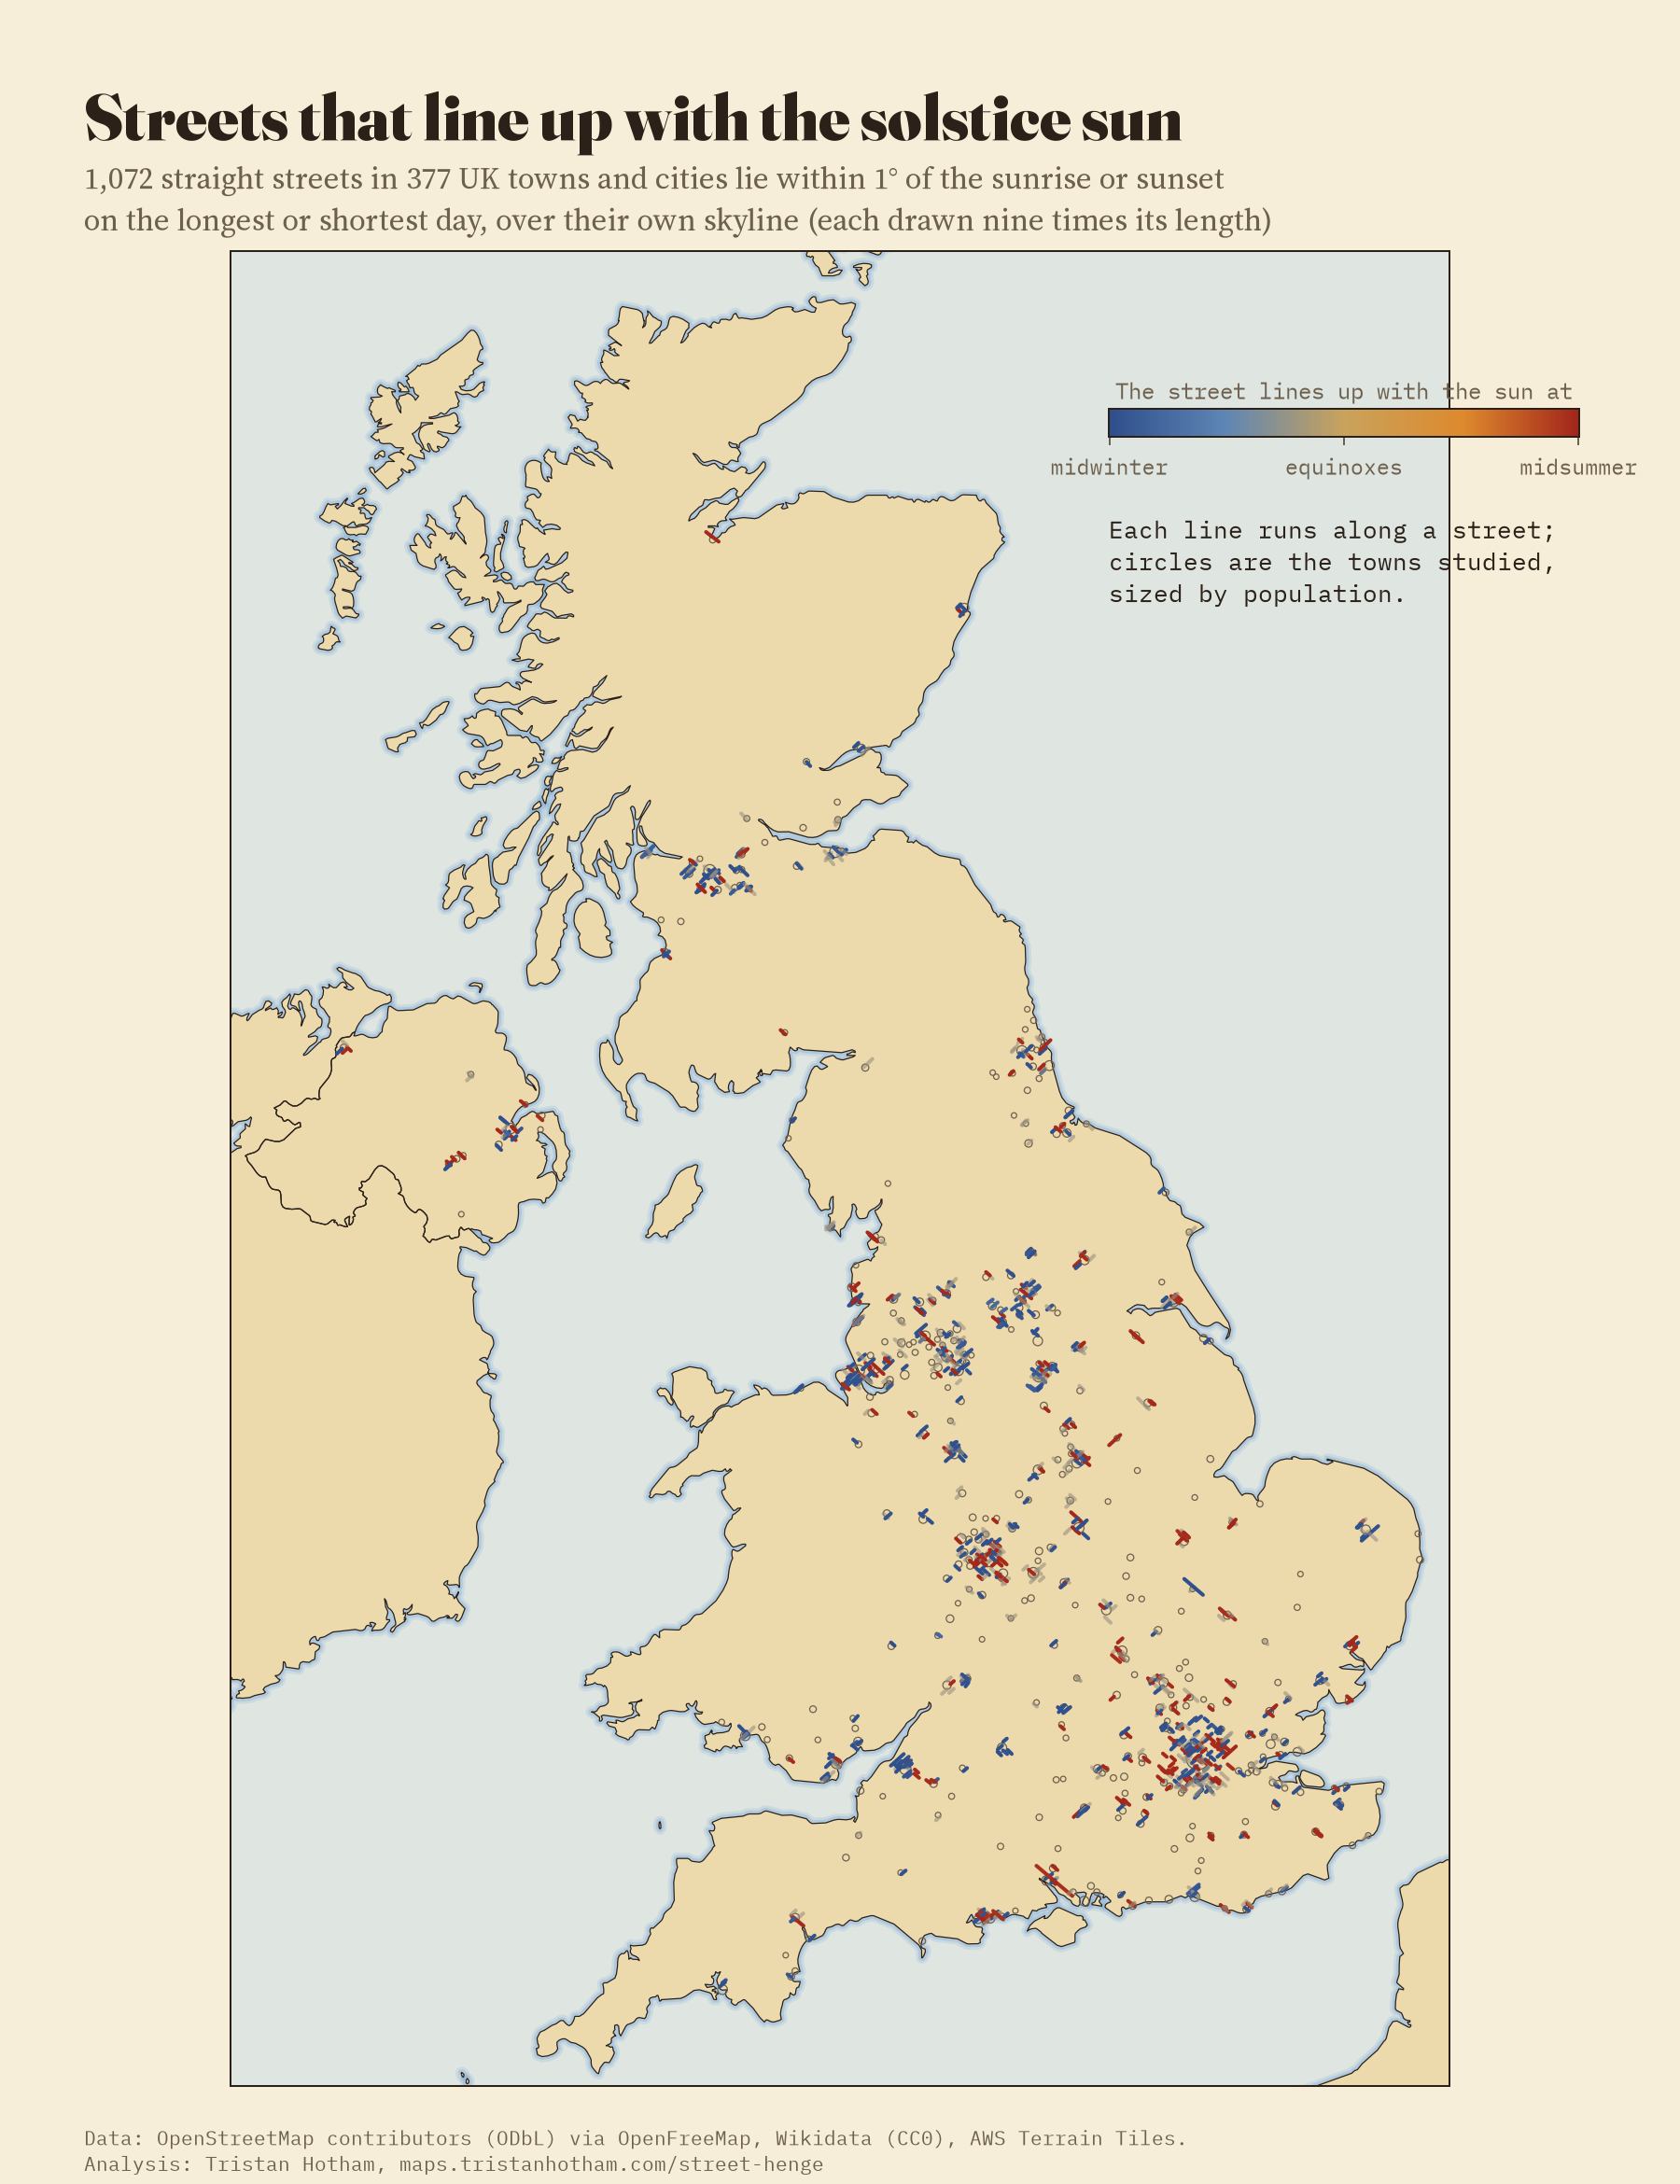
\includegraphics[width=0.78\textwidth]{f_map.png}
\caption{Streets within 1° of a solstice sunrise or sunset, drawn nine times their length and coloured by the declination at which the sun lines up.}\label{fig:map}\end{figure}
\begin{figure}[tbp]\centering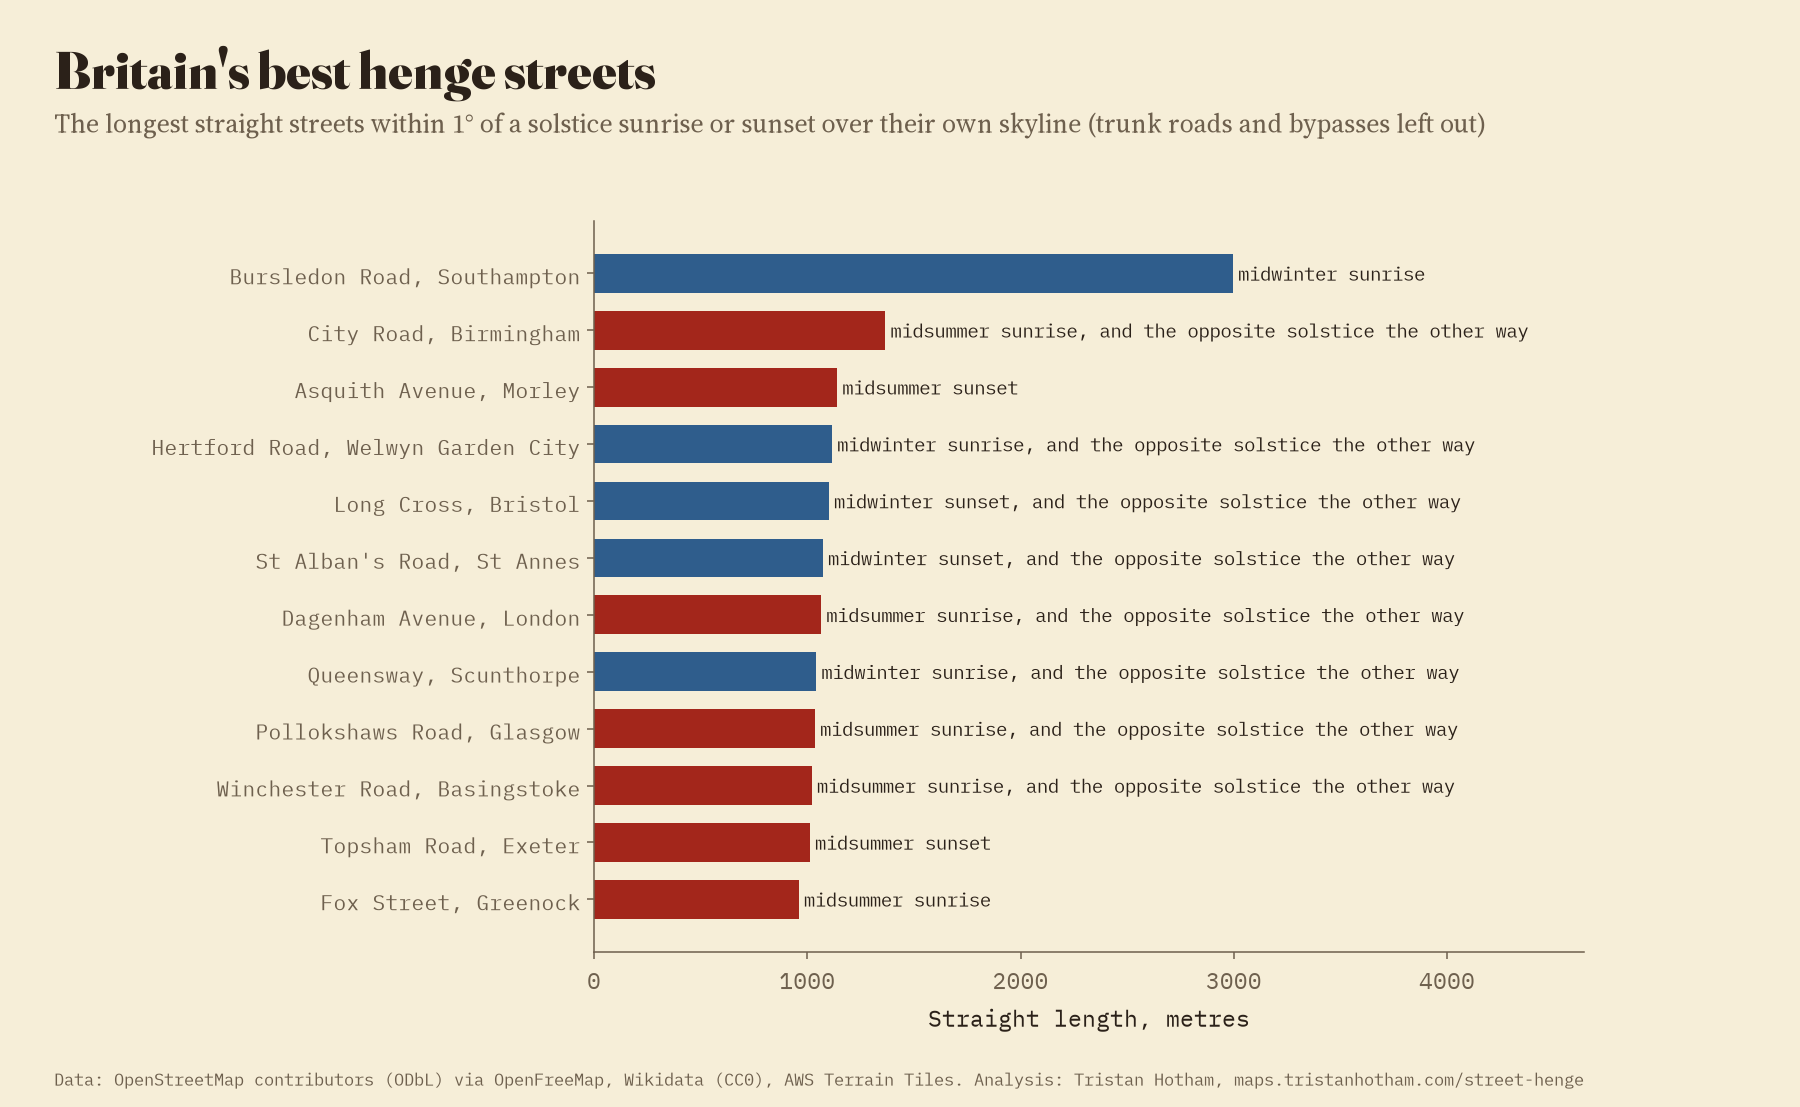
\includegraphics[width=0.92\textwidth]{f_best.png}
\caption{The longest solstice-aligned streets (trunk roads and bypasses excluded).}\label{fig:best}\end{figure}

\subsection{Chance}
Across all 74,448 street ends, 1,383 (1.86\%) lie within 1° of a solstice azimuth, against 1.83\% expected from the neighbouring offsets (ratio 1.01, p = 0.31; Figure~\ref{fig:chance}). The distribution of offsets is flat through zero. Of 168 towns tested, 3 have significantly more solstice ends than expected after correction: St Annes (21 against 3.2), Bournemouth (22 against 6.8) and Basingstoke (13 against 3.7). These are local grids that happen to run near a solstice line; nothing in the data shows the sun was the reason.

\begin{figure}[tbp]\centering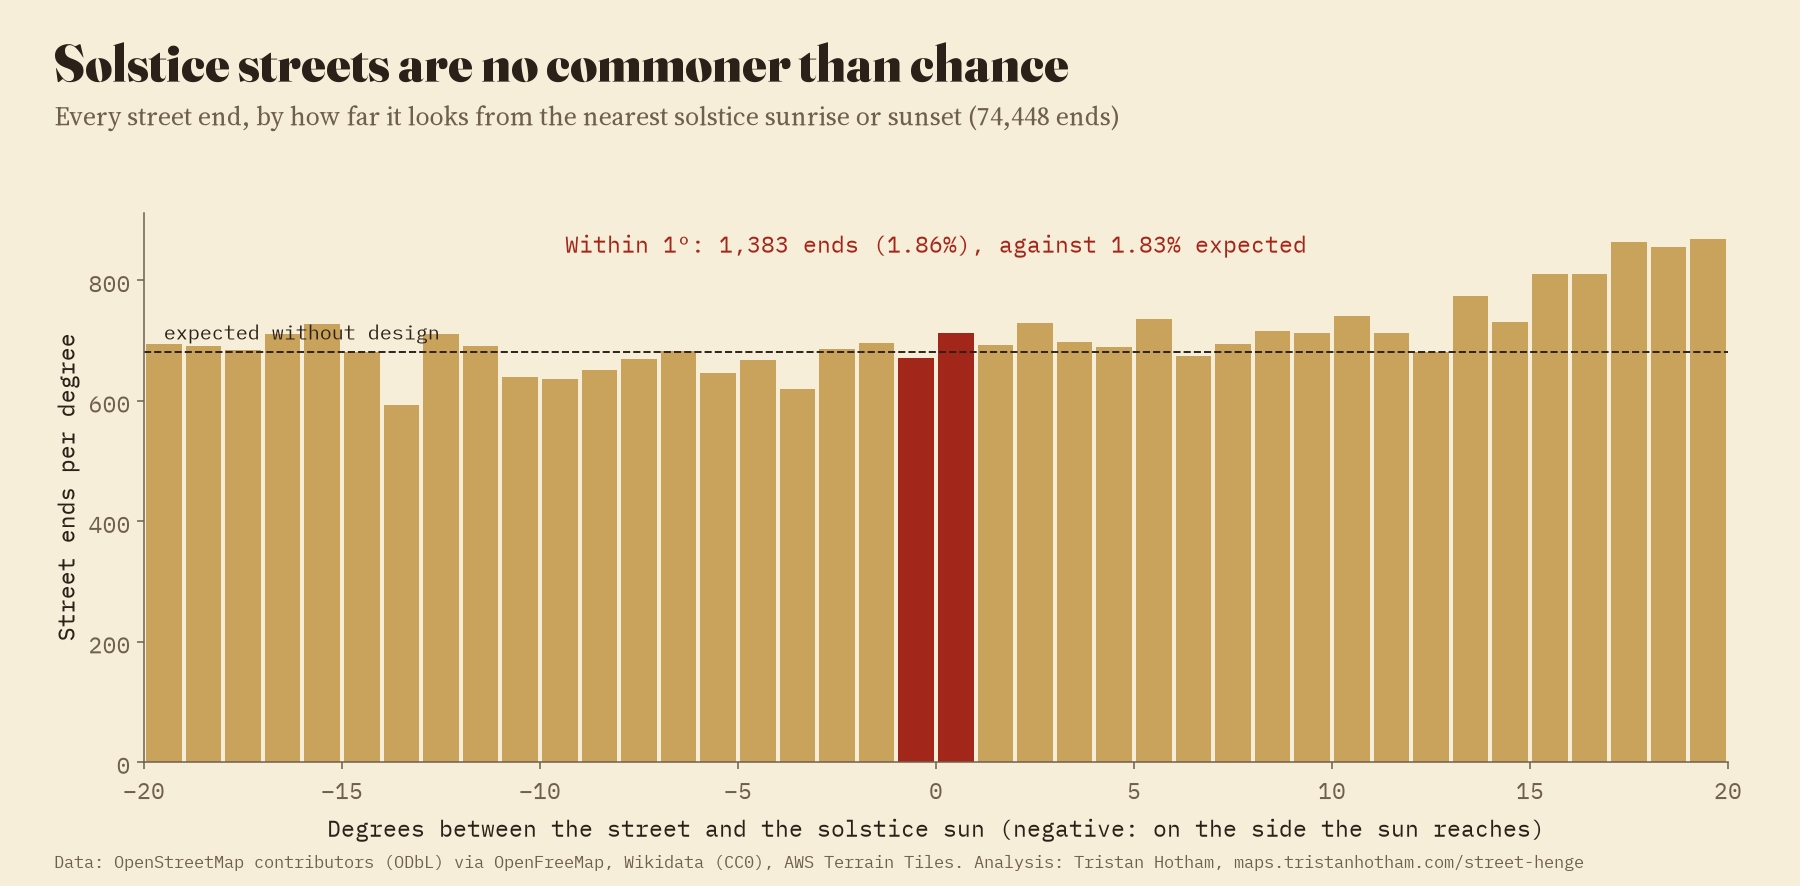
\includegraphics[width=\textwidth]{f_chance.png}
\caption{Street ends by their angle from the nearest solstice sunrise or sunset; the dashed line is the expectation from offsets of 2° to 8°.}\label{fig:chance}\end{figure}

\subsection{Milton Keynes}
Midsummer Boulevard is mapped as 2 straight stretches (1.26 km) with a length-weighted bearing of 55.1°. The midsummer sun rises over its eastern skyline (between -0.1° and 1.2°) at about 50.1°, and at 48.7° over a flat horizon, so the boulevard misses it by 4.0° to 6.7° (Figure~\ref{fig:mk}). The sun rises along it about 24 May and 20 July. The town's grid runs at 59.1° (strength 0.34) and 7 of its 233 stretches are solstice aligned. An independent check of the mapped geometry gives the same direction: each of the boulevard's 8 mapped pieces longer than 150 m, read straight from the tiles, runs at 54.8° to 56.4° from true north on the ellipsoid (55.2° along the principal axis of all its vertices). Measured on the Ordnance Survey National Grid, whose north here lies 1.0° east of true north, the same line reads 1.0° less, so a bearing taken from a grid map understates the miss slightly. The midsummer sun's upper limb first appears over a flat horizon at 48.2° and its centre at 48.7° (independently, 48.2° and 48.8° with PyEphem for 21 June 2026, which also puts the sun on the axis 3.6° up, 35 minutes after the first gleam). A misalignment of this size is far larger than the uncertainty of the mapped centreline or the skyline.

What the planners claimed was more modest than the popular story. David Lock, the planner of the city centre, is quoted as saying that the road could be called Midsummer Boulevard because people could be told that on Midsummer's Day the sun rises at the end of it, ``which it nearly does'' \citep{hill}; Stuart Mosscrop, the chief architect, said the first match with the solstice was a coincidence and that the grid was then rearranged slightly to line up \citep{parks}. The later account of an exact angle supplied by the Greenwich observatory is not borne out by the street. What holds is that on midsummer morning the sun's centre stands on the axis at an apparent altitude of 3.6°, about 36 minutes after the first gleam. From the low western end near the station, looking up the boulevard, the terrain alone rises to 1.2°, and the trees and buildings on the crest, which the terrain model does not contain, raise the skyline further, towards the altitude at which the sun is on the axis; a viewer there can see the sun clear the crest on the line of the road. From the open eastern end the midsummer sun rises 6.7° to the left of the axis. The Parks Trust itself notes that the sun rises in line with the boulevard on 20 July \citep{parks}, as found here.

\begin{figure}[tbp]\centering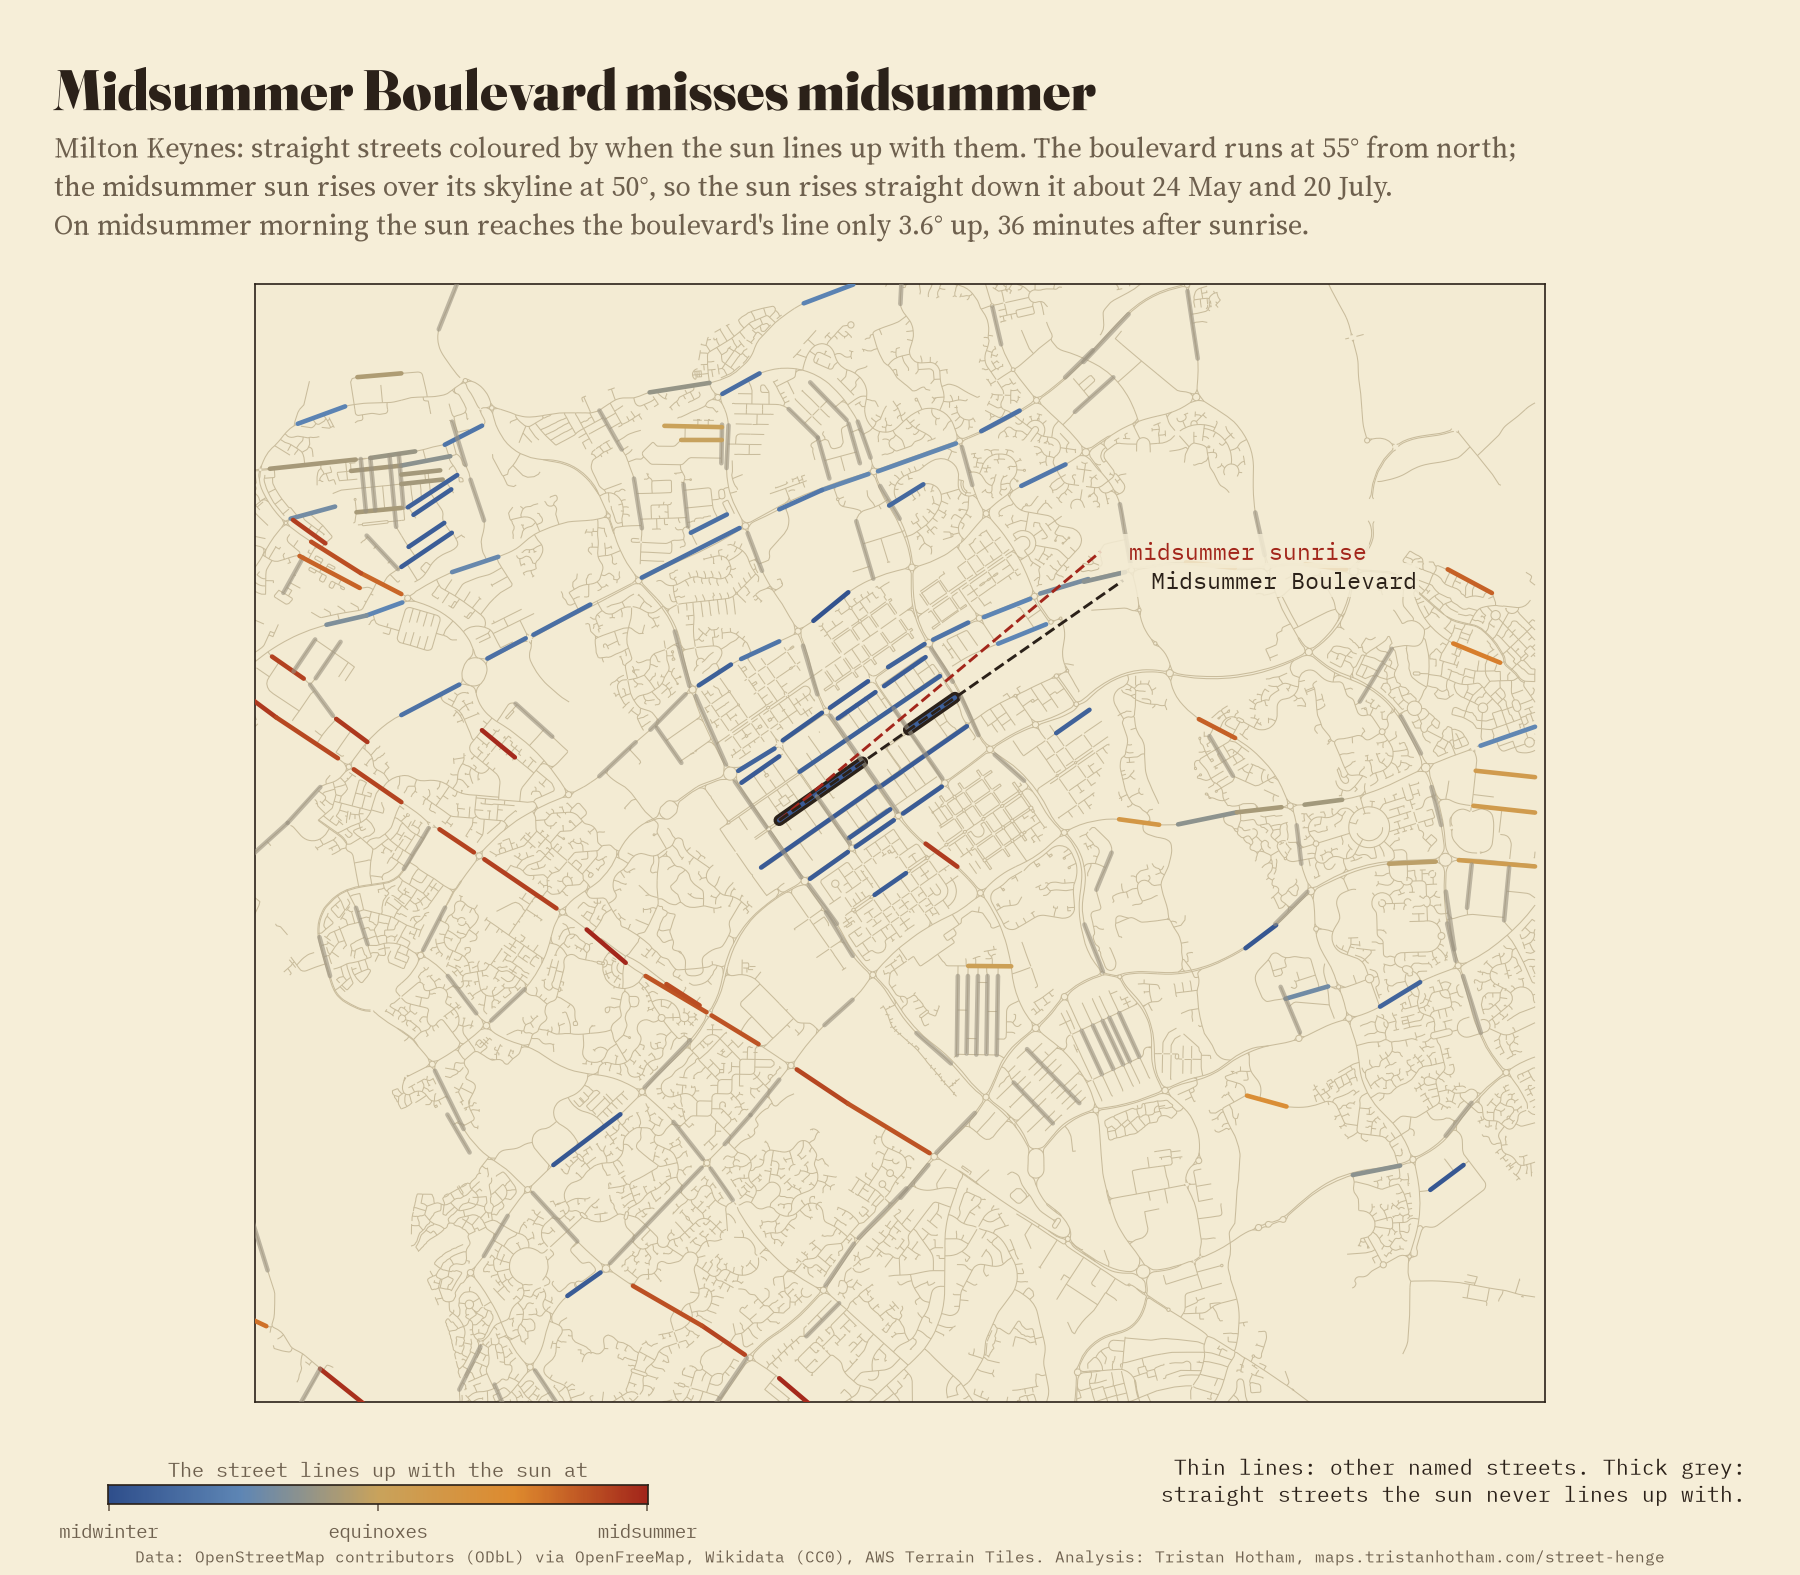
\includegraphics[width=0.85\textwidth]{f_mk.png}
\caption{Milton Keynes: straight streets coloured by the declination at which the sun lines up, and the lines of Midsummer Boulevard and the midsummer sunrise.}\label{fig:mk}\end{figure}

\subsection{Henge calendars and grids}
Table~\ref{tab:cities} gives the best henge days and grid of the largest cities, and Figures~\ref{fig:calendars} and \ref{fig:grids} show calendars and grids. Glasgow's grid, turned 8.7° from north with strength 0.34, gives sunsets along its east to west streets in early April and mid September; Edinburgh's New Town grid (74.7°) gives sunsets in late February and mid October. The strongest grids are in seaside towns laid out square to the shore, led by Great Yarmouth (strength 0.83) and Worthing (0.80), whose streets catch the sun near the equinoxes.

\begin{table}[tbp]\centering\small\caption{The largest cities: straight stretches, their length (km), solstice-aligned stretches, grid direction (degrees, modulo 90) and strength, and the best henge day with its near-equal twin on the other side of the solstice.}\label{tab:cities}\begin{tabular}{lrrrrrl}\toprule City & Stretches & km & Solstice & Grid & Strength & Best days\\\midrule
London & 6,349 & 2634 & 151 & 78.7 & 0.18 & 12 April, 1 September (sunrise)\\
Birmingham & 1,370 & 575 & 41 & 7.0 & 0.04 & 18 March, 22 September (sunset)\\
Glasgow & 968 & 414 & 14 & 8.7 & 0.34 & 6 April, 7 September (sunset)\\
Manchester & 741 & 333 & 16 & 85.6 & 0.18 & 21 April, 22 August (sunrise)\\
Leeds & 575 & 242 & 15 & 6.1 & 0.13 & 8 March, 6 October (sunrise)\\
Liverpool & 870 & 376 & 27 & 67.5 & 0.24 & 24 February, 18 October (sunset)\\
Edinburgh & 518 & 216 & 9 & 74.7 & 0.38 & 1 September, 12 April (sunrise)\\
Bristol & 372 & 152 & 19 & 48.1 & 0.08 & 18 April, 26 August (sunset)\\
Cardiff & 339 & 138 & 11 & 54.4 & 0.08 & 25 January, 16 November (sunset)\\
Belfast & 418 & 182 & 14 & 22.6 & 0.14 & 21 February, 21 October (sunrise)\\
Newcastle upon Tyne & 465 & 193 & 8 & 85.8 & 0.27 & 21 March, 23 September (sunrise)\\
Sheffield & 539 & 226 & 21 & 61.2 & 0.09 & 30 March, 14 September (sunset)\\
Milton Keynes & 233 & 99 & 7 & 59.1 & 0.34 & 19 January, 24 November (sunset)\\
\bottomrule\end{tabular}\end{table}

\begin{figure}[tbp]\centering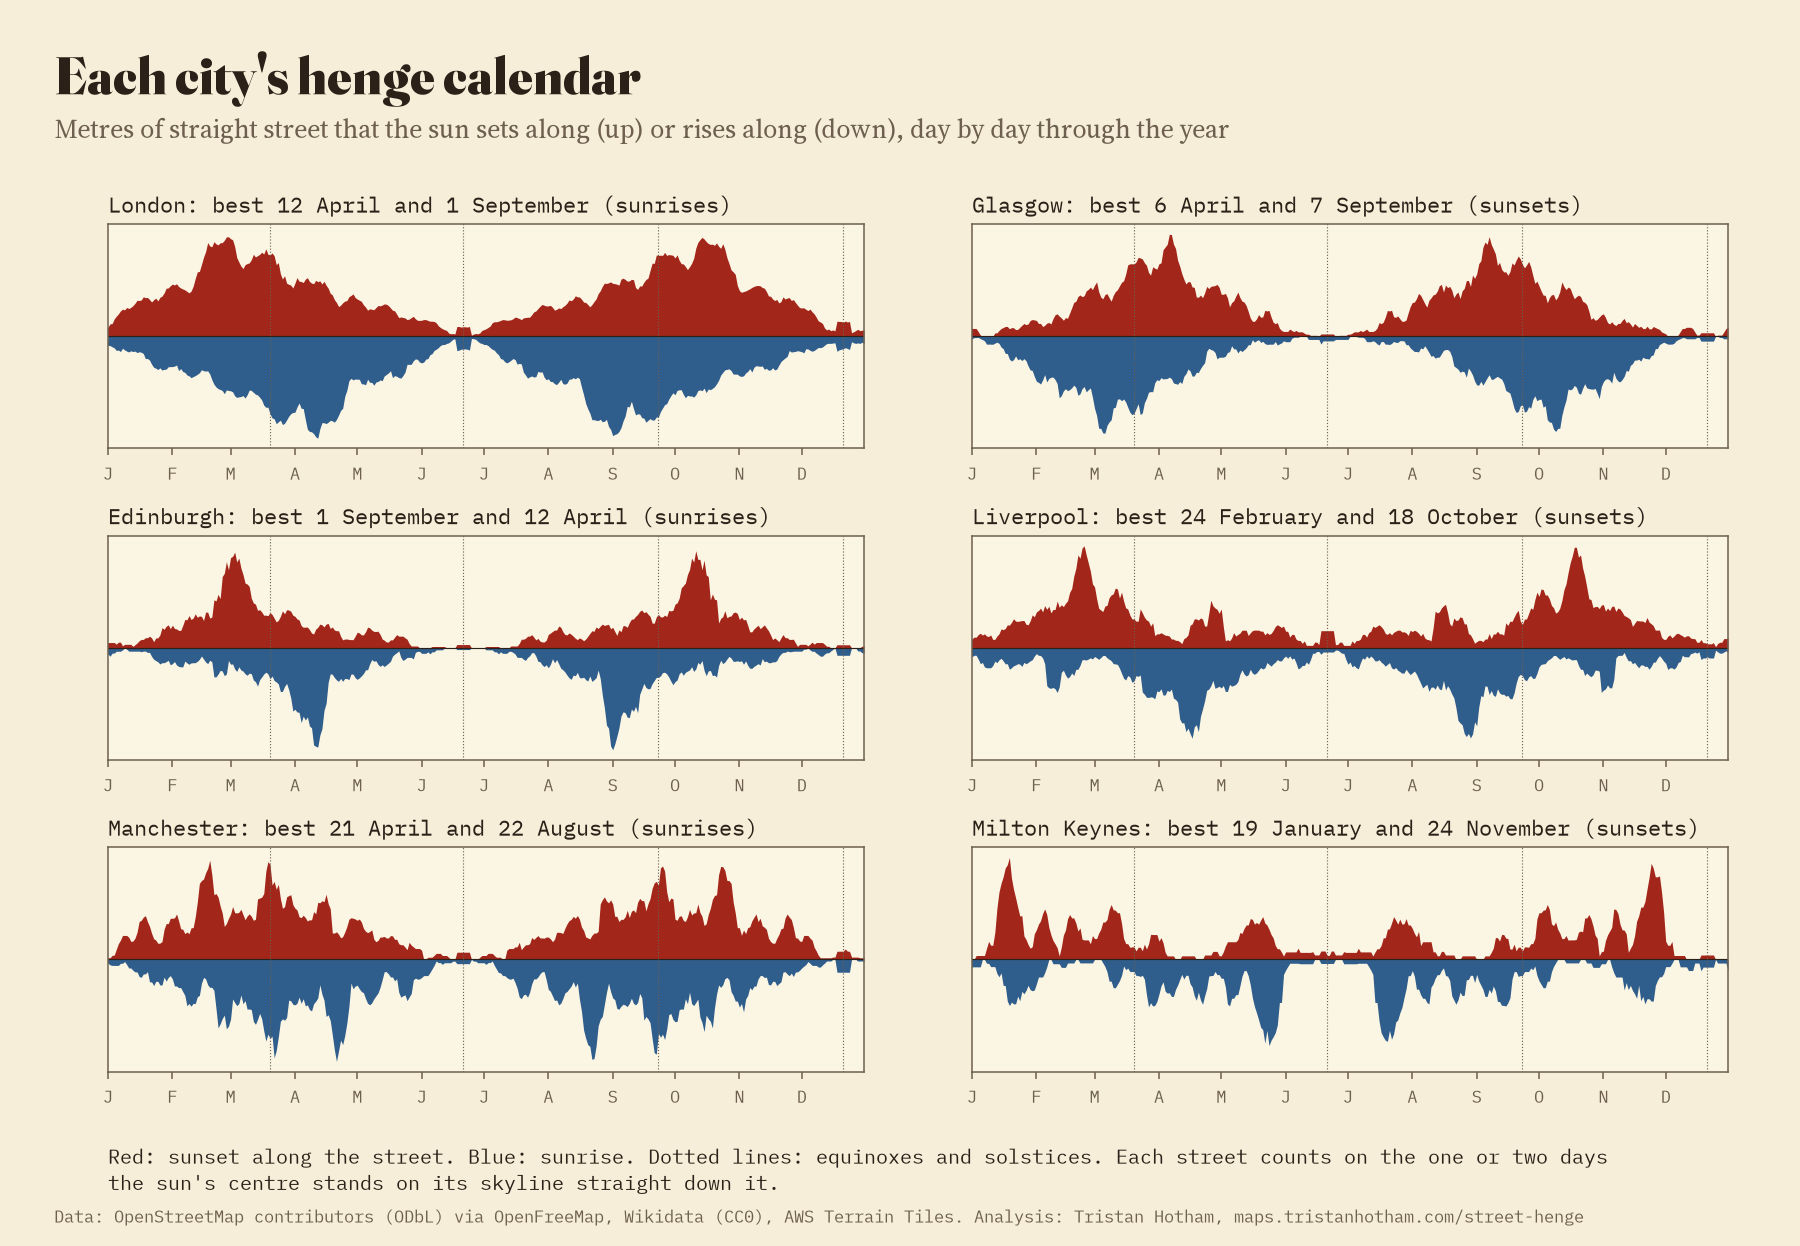
\includegraphics[width=\textwidth]{f_calendars.png}
\caption{Henge calendars: metres of straight street the sun sets along (up) or rises along (down), by day of the year.}\label{fig:calendars}\end{figure}
\begin{figure}[tbp]\centering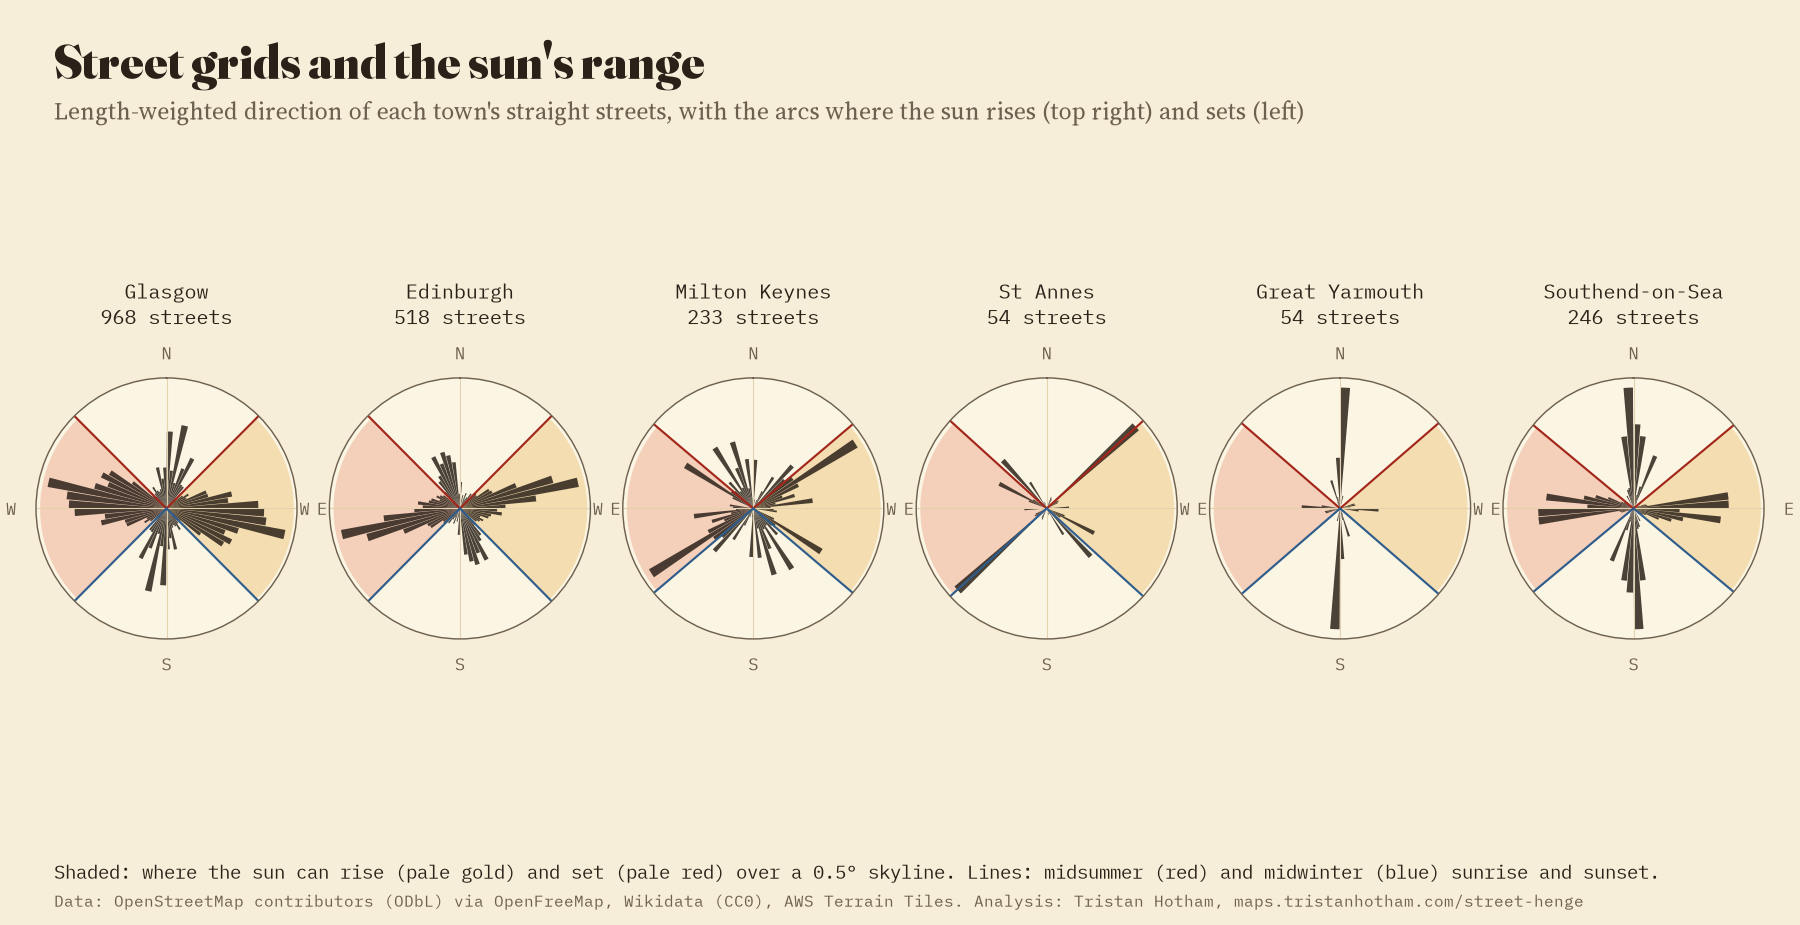
\includegraphics[width=\textwidth]{f_grids.png}
\caption{Length-weighted street directions in six towns, over the arcs of sunrise and sunset.}\label{fig:grids}\end{figure}

\section{Limitations}
Buildings, trees and the curve of a street beyond the straight stretch are not modelled: the skyline is the terrain's, so many alignments will be blocked in practice, and the most dramatic henges (a long street open to a low horizon) are not distinguished from streets that end at a wall. The 5 m tolerance allows a bearing error of about 1° on the shortest stretches. OpenStreetMap centrelines are generally accurate to a few metres in towns, but mapped geometry can be simplified in the vector tiles. Dates depend on the definition of the moment (here the sun's centre on the skyline; the first gleam of the upper limb is about 0.5° further from the meridian at midsummer in the UK) and move by up to a day between years. The two ends of a street are not independent (a street aligned at one end with the midsummer sunrise often meets the midwinter sunset at the other), so the binomial tests treat correlated ends as separate; allowing for the observed correlation does not change any conclusion. Town circles are crude, and the population threshold leaves out smaller planned places. The chance test can detect a general preference for solstice alignment, but not the intention behind a single street.

\section{Conclusion}
Half of Britain's straight town streets catch the rising or setting sun on some day of the year, and every town has its henge days, which can be looked up on the map. About a thousand line up with a solstice, but no more than chance would give; Britain's streets were not laid out to the sun. Midsummer Boulevard, the famous case, misses the midsummer sunrise over the land by several degrees; it lines up with the midsummer sun only once the sun is a few degrees up, as seen over the rise from its western end, which is roughly what its planners said.

\section*{Data and code availability}
The interactive map is at \url{https://maps.tristanhotham.com/street-henge/}. Data and code are at \url{https://github.com/Tristan-Hotham/street-henge} and archived with this paper at https://doi.org/10.5281/zenodo.24075297. The street table is derived from OpenStreetMap and released under the Open Database Licence; Wikidata is CC0; code is MIT licensed; text and figures CC BY 4.0.

\section*{AI statement}
I wrote the text, with drafting and editing assistance from Claude (Anthropic), which also helped prepare the analysis code. I reviewed and checked all text and results.

\begin{thebibliography}{99}
\bibitem[Bennett(1982)]{bennett} Bennett, G. G. (1982) The calculation of astronomical refraction in marine navigation. \textit{Journal of Navigation} 35(2), 255 to 259.
\bibitem[Boeing(2019)]{boeing} Boeing, G. (2019) Urban spatial order: street network orientation, configuration, and entropy. \textit{Applied Network Science} 4, 67.
\bibitem[Hill(2007)]{hill} Hill, M. (ed.) (2007) \textit{The Story of the Original Central Milton Keynes}. Milton Keynes: Living Archive.
\bibitem[OpenFreeMap(2026)]{ofm} OpenFreeMap (2026) Free vector tiles (OpenMapTiles schema) from OpenStreetMap data. \url{https://openfreemap.org/}
\bibitem[OpenStreetMap contributors(2026)]{osm} OpenStreetMap contributors (2026) OpenStreetMap. Open Database Licence. \url{https://www.openstreetmap.org/}
\bibitem[The Parks Trust(n.d.)]{parks} The Parks Trust (n.d.) Mysticism in the park. Campbell Park heritage trail. \url{https://theparkstrust.com/our-work/heritage/campbell-park-trail/mysticism-in-the-park}
\bibitem[Spencer(1971)]{spencer} Spencer, J. W. (1971) Fourier series representation of the position of the sun. \textit{Search} 2(5), 172.
\bibitem[Tilezen(2026)]{terrain} Tilezen / Mapzen (2026) Terrain Tiles on AWS (Registry of Open Data). \url{https://registry.opendata.aws/terrain-tiles/}
\bibitem[Wikidata(2026)]{wikidata} Wikidata contributors (2026) Wikidata. CC0. \url{https://www.wikidata.org/}
\end{thebibliography}

\end{document}
